\documentclass{include/thesisclass}
% Main File - Based on thesisclass.cls
% Comments are mostly in English
% ------------------------------------------------------------------------------
% Further files in folder:
%  - include/cmds.tex (for macros and additional commands)
%  - include/kitlogo.pdf (for titlepage)
%  - lit.bib (bibtex bibliography database)
%  - include/titlepage.tex (for layout of titelpage)
% ------------------------------------------------------------------------------
% Useful Supplied Packages:
% amsmath, amssymb, mathtools, bbm, upgreek, nicefrac,
% siunitx, varioref, booktabs, graphicx, tikz, multicol





%% -------------------------
%% |    Thesis Settings    |
%% -------------------------
% english or ngerman (new german für neue deutsche Rechtschreibung statt german)
\SelectLanguage{english}
% details on this thesis
\newcommand{\thesisauthor}{Chenran Xu}
\newcommand{\thesistopic}{Untersuchung der Langzeitstabilität des EDELWEISS Myon-Veto-Systems}
\newcommand{\thesisentopic}{Investigation of the long term stability of the EDELWEISS muon veto system}
\newcommand{\thesislongtopic}{Very long and very detailed description of the very interesting thesis topic (only necessary for pdfsubject tag).}
\newcommand{\thesisinstitute}{Institut für Experimentelle Kernphysik}
\newcommand{\thesisreviewerone}{Prof. Dr. D. Cay}
\newcommand{\thesisreviewertwo}{Prof. Dr. E. Vil}
\newcommand{\thesisadvisorone}{} % to use: enter names and uncomment in titlepg
\newcommand{\thesisadvisortwo}{}
\newcommand{\thesistimestart}{01.04.2015} % on titlepage
\newcommand{\thesistimeend}{30.09.2015} % on titlepage
\newcommand{\thesistimehandin}{30.09.2015} % on second page 'preamble'
\newcommand{\thesispagehead}{Bachelor Thesis: \thesisentopic} % page heading





%% ---------------------
%% |    PDF - Setup    |
%% ---------------------
% This information will appear embed into the PDF file as meta data, but will
% not be printed anywhere
\hypersetup
{
    pdfauthor={\thesisauthor},
    pdftitle={Bachelorarbeit: \thesistopic},
    pdfsubject={\thesislongtopic},
    pdfkeywords={kit,physik,bachelor,thesis,\thesisauthor}
}





%% --------------------------------------
%% |    Settings for Word Separation    |
%% --------------------------------------
% Help for separation:
% In German package the following hints are additionally available:
% "- = Additional separation
% "| = Suppress ligation and possible separation (e.g. Schaf"|fell)
% "~ = Hyphenation without separation (e.g. bergauf und "~ab)
% "= = Hyphenation with separation before and after
% "" = Separation without a hyphenation (e.g. und/""oder)

% Describe separation hints here:
\hyphenation
{
    über-nom-me-nen an-ge-ge-be-nen
    %Pro-to-koll-in-stan-zen
    %Ma-na-ge-ment  Netz-werk-ele-men-ten
    %Netz-werk Netz-werk-re-ser-vie-rung
    %Netz-werk-adap-ter Fein-ju-stier-ung
    %Da-ten-strom-spe-zi-fi-ka-tion Pa-ket-rumpf
    %Kon-troll-in-stanz
}





%% -----------------------
%% |    Main Document    |
%% -----------------------
\usepackage{lipsum} % for Lorem Ipsum text example
\begin{document}
    % Titlepage and ToC
    \FrontMatter

    % coordinates for background border
\newcommand{\diameter}{20}
\newcommand{\xone}{-15}
\newcommand{\xtwo}{160}
\newcommand{\yone}{15}
\newcommand{\ytwo}{-253}




\begin{titlepage}
    % background border
    \begin{tikzpicture}[overlay]
    \draw[color=gray]
            (\xone mm, \yone mm)
      -- (\xtwo mm, \yone mm)
    arc (90:0:\diameter pt)
      -- (\xtwo mm + \diameter pt , \ytwo mm)
        -- (\xone mm + \diameter pt , \ytwo mm)
    arc (270:180:\diameter pt)
        -- (\xone mm, \yone mm);
    \end{tikzpicture}



    % KIT image and sign for faculty of physics
    \begin{textblock}{10}[0,0](4.5,2.5)
        
\includegraphics[width=.25\textwidth]{include/kitlogo.pdf}
    \end{textblock}
    \changefont{phv}{m}{n}    % helvetica
    \begin{textblock}{10}[0,0](5.5,2.2)
        \begin{flushright}
            \Large FAKULTÄT FÜR PHYSIK\\\thesisinstitute
        \end{flushright}
    \end{textblock}



    % horizontal line
    \begin{textblock}{10}[0,0](4.2,3.1)
        \begin{tikzpicture}[overlay]
        \draw[color=gray]
                (\xone mm + 5 mm, -12 mm)
          -- (\xtwo mm + \diameter pt - 5 mm, -12 mm);
        \end{tikzpicture}
    \end{textblock}



    % begin of text part
    \changefont{phv}{m}{n}    % helvetica
    \centering



    % thesis topic (en and ge)
    \vspace*{3cm}
    \Huge\thesistopic\\
    \huge(\thesisentopic)\\



    % author name and institute
    \vspace*{2cm}
    \Large Bachelorarbeit\\von\\
    \vspace*{1cm}
    \huge\thesisauthor\\
    \vspace*{1cm}
    \Large am \thesisinstitute



    % possible frontimage - thanks to JabberWok
    % for publishing the img under GNU Document License
    \vspace*{1.5cm}
 	%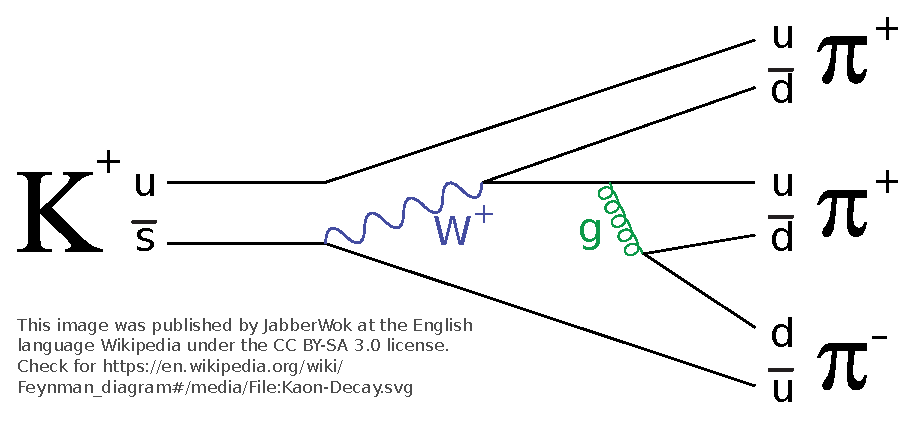
\includegraphics[scale=0.7]{./include/frontimage.eps}
 	


    % examiners (Referenten)
    \vspace*{1.5cm}
    \Large
    \begin{center}
        \begin{tabular}[ht]{l c l}
        \iflanguage{english}{Reviewer}{Referent}: 
            & \hfill & \thesisreviewerone\\
        \iflanguage{english}{Second Reviewer}{Korreferent}: 
            & \hfill & \thesisreviewertwo\\
        % uncomment if you want to provide info on your advisors
        %\iflanguage{english}{Advisor}{Betreuender Mitarbeiter}: 
        %    & \hfill & \thesisadvisorone\\
        %\iflanguage{english}{Second Advisor}{Zweiter betreuender Mitarbeiter}: 
        %    & \hfill & \thesisadvisortwo\\
        \end{tabular}
    \end{center}



    % working time
    \vspace{1cm}
    \begin{center}
        \large{{Bearbeitungszeit}: \thesistimestart \hspace*{0.25cm} -- %
                                   \hspace*{0.25cm} \thesistimeend}
    \end{center}



    % lowest text blocks concerning the KIT
    \begin{textblock}{10}[0,0](4,16.8)
        \tiny{KIT -- Universität des Landes Baden-Württemberg und nationales %
              Forschungszentrum in der Helmholtz-Gemeinschaft}
    \end{textblock}
    \begin{textblock}{10}[0,0](14,16.75)
        \large{\textbf{www.kit.edu}}
    \end{textblock}
\end{titlepage}

    \chapter*{Erklärung zur Selbstständigkeit}
Ich versichere, dass ich diese Arbeit selbstständig verfasst habe und keine %
anderen als die angegebenen Quellen und Hilfsmittel benutzt habe, die %
wörtlich oder inhaltlich übernommenen Stellen als solche kenntlich gemacht und %
die Satzung des KIT zur Sicherung guter wissenschaftlicher Praxis in der %
gültigen Fassung vom 17.05.2010 beachtet habe.\\

\vspace{1cm}

\renewcommand{\arraystretch}{0} % for spacing in the tabular environment

\begin{flushright}
	\begin{tabular}{rr}
		Karlsruhe, den \thesistimehandin, & \hspace*{5cm}\\[0mm]
		\cline{2-2}\\[2mm]    % the last line has height 2mm due
		& \thesisauthor       % to \arraystretch=0
	\end{tabular}
\end{flushright}

\vfill

\begin{flushright}
	Als Ansichtsexemplar genehmigt von\\
	\vspace{1cm}
	\begin{tabular}{rr}
		Karlsruhe, den \thesistimehandin, & \hspace*{5cm}\\[0mm]
		\cline{2-2}\\[2mm]    % the last line has height 2mm due
		& \thesisreviewerone  % to \arraystretch=0
	\end{tabular}
\end{flushright}

\renewcommand{\arraystretch}{1}

\cleardoublepage


    \begingroup \let\clearpage\relax    % in order to avoid listoffigures and
    \tableofcontents                    % listoftables on new pages
    \listoffigures
    \listoftables
    \endgroup
    \cleardoublepage



    % Contents
    \MainMatter

    \chapter{Introduction}
    some introduction &
    outline
    \chapter{WIMPs-search with EDELWEISS-III Experiment}
      \section{Evidences of dark matter}
      kinematic, interaction.
      \section{WIMP as dark matter candidate}

      \section{EDELWEISS-III Experiment}
        \subsection{Experimental setup}
        \subsection{Backgrounds at EDELWEISS Experiment}

    \chapter{Detection of muons in EDELWEISS-III Experiment}
      \section{Muon veto system}
        \subsection{Experimental setup}
        \subsection{Energy deposit of muon in the scintillator module}
        \subsection{Working Principle}
          electronics

    \chapter{Analysis of the long term measurement data}
      \section{(Determination of the aging effect using) LED events}
        \subsection{Data selection}
          cut criterium
        \subsection{}

      \section{Muon events}
        \subsection{Data selection}
        \subsection{Analysis of MPV of Landau-Specturm}
      \section{Muon Detection Efficiency}
        \subsection{Effective trigger threshold}
         methods used,
    \chapter{Conclusions}




    %\emptychapter[3]{ROOT Routines}     % usage: \emptychapter[page displayed
                                        %        in toc]{name of the chapter}


    % appendix for more or less interesting calculations
    \Appendix
    \chapter*{\appendixname} \addcontentsline{toc}{chapter}{\appendixname}
    % to make the appendix appear in ToC without number. \appendixname =
    % Appendix or Anhang (depending on chosen language)
    % \section{Detection Efficiency}
\label{sec:appendix}
some text!
%tables of efficiency
\small
\begin{longtable}{c c c c c c c c c}
  \caption{The determined trigger threshold and detection efficiency of each module in Run70-79 (2010). For some PMT groups, the spectrum cannot be fitted properly and no efficiency value can be derived. The detection efficiency is estimated by the other PMT group in the same module, or the mean value of the modules on the same side if both spectra of PMT groups cannot be fitted. } \\
  \label{tab:mpv-full}\\
  \toprule
  Module & End & MPV & Threshold & $\sigma{}_{\mathrm{erf}}$ & $\epsilon_{20\%}$ & $\epsilon_{50\%\mathrm{MPV}}$ & $\epsilon_{\mathrm{MPV}}$ & $\epsilon_{\mathrm{tot}, 50\%\mathrm{MPV}}$ \\
         &     & \multicolumn{3}{|c|}{in ADC channels} &   \\
  \midrule
  \endfirsthead
  Top\\
  \midrule
  M1 & N & 1036 & 939 & 690 & 0.66 & 0.65 & 0.80 & \multirow{2}{*}{0.4}\\
     & S & 827 & 191 & 2193 & 0.69 & 0.71 & 0.75 & \\
  M2 & N & 625 & 786 & 1622 & 0.56 & 0.60 & 0.66 & \multirow{2}{*}{0.33}\\
     & S & 214 & 829 & 1905 & 0.53 & 0.55 & 0.57 & \\
  M3 & N & 647 & 494 & 98 & 0.88 & 0.83 & 1.00   & \multirow{2}{*}{0.75}\\
     & S & 918 & 635 & 136 & 0.90 & 0.90 & 1.00  & \\
  M4 & N & 352 & 880 & 194 &   &   &             & \multirow{2}{*}{0.71}\\
     & S & 355 & 890 & 157 &   &   &             & \\
  M5 & N & 1197 & 554 & 865 & 0.79 & 0.84 & 0.93 & \multirow{2}{*}{0.70}\\
     & S & 1108 & 645 & 607 & 0.78 & 0.83 & 0.94 & \\
  M6 & N & 1401 & 532 & 737 & 0.86 & 0.90 & 0.97 & \multirow{2}{*}{0.77}\\
     & S & 1256 & 615 & 712 & 0.83 & 0.86 & 0.95 & \\
  M7 & N & 1080 & 190 & 366 & 0.97 & 0.99 & 1.00 & \multirow{2}{*}{0.98}\\
     & S & 941 & 202 & 223 & 0.98 & 0.99 & 1.00  & \\
  M8 & N & 1443 & 638 & 155 & 0.99 & 0.99 & 1.00 & \multirow{2}{*}{0.99}\\
     & S & 2217 & 251 & 101 & 0.98 & 1.00 & 1.00 & \\
  \midrule
  N1-North\\
  \midrule
  M9 & ADC[0] & 1320 & 751 & 791 & 0.71 & 0.82 & 0.93 & \multirow{2}{*}{0.80}\\
     & ADC[1] & 3000 & 100 & 1282 & 0.86 & 0.97 & 1.00 &\\
  M10 & ADC[0] & 650 & 476 & 910 & 0.68 & 0.76 & 0.84 & \multirow{2}{*}{0.71}\\
      & ADC[1] & 1410 & 100 & 989 & 0.87 & 0.93 & 0.98 & \\
  M11 & ADC[0] & 1133 & 685 & 409 & 0.82 & 0.86 & 0.98 & \multirow{2}{*}{0.83}\\
      & ADC[1] & 952 & 493 & 176 & 0.94 & 0.97 & 1.00 & \\
  M12 & ADC[0] & 881 & 660 & 120 & 0.92 & 0.86 & 1.00 & \multirow{2}{*}{0.86}\\
      & ADC[1] & 1140 & 395 & 146 & 0.97 & 1.00 & 1.00 &\\
  M13 & ADC[0] & 799 & 122 & 1184 & 0.79 & 0.85 & 0.90 & \multirow{2}{*}{0.80}\\
      & ADC[1] & 1331 & 298 & 784 & 0.84 & 0.94 & 0.98 & \\
  M14 & ADC[0] & 1118 & 836 & 489 & 0.73 & 0.75 & 0.92 & \multirow{2}{*}{0.61}\\
      & ADC[1] & 1138 & 100 & 1729 & 0.77 & 0.82 & 0.87 & \\
  M15 & ADC[0] & 2674 & 560 & 143 & 0.99 & 1.00 & 1.00 & \multirow{2}{*}{1.00}\\
      & ADC[1] & 1292 & 186 & 13 & 1.00 & 1.00 & 1.00\\
  \midrule
  N1-South\\
  \midrule
  M16 & ADC[0] & 2481 & 267 & 91 & 0.99 & 1.00 & 1.00 & \multirow{2}{*}{1.00}\\
      & ADC[1] & 2451 & 296 & 103 & 0.98 & 1.00 & 1.00 &\\
  M17 & ADC[0] & 1200 & 515 & 112 & 0.99 & 1.00 & 1.00 & \multirow{2}{*}{0.94}\\
      & ADC[1] & 1043 & 100 & 740 & 0.88 & 0.94 & 0.98 &\\
  M18 & ADC[0] & 893 & 692 & 1254 & 0.65 & 0.69 & 0.78 & \multirow{2}{*}{0.69}\\
      & ADC[1] & 2184 & 517 & 153 & 0.97 & 1.00 & 1.00 & \\
  M19 & ADC[0] & 1207 & 587 & 146 & 0.97 & 0.98 & 1.00 & \multirow{2}{*}{0.98}\\
      & ADC[1] & 1799 & 533 & 146 & 0.99 & 1.00 & 1.00 & \\
  M20 & ADC[0] & 2133 & 1352 & 1343 & 0.55 & 0.72 & 0.87 & \multirow{2}{*}{0.63}\\
      & ADC[1] & 1476 & 687 & 639 & 0.74 & 0.90 & 0.98 & \\
  M21 & ADC[0] & 1117 & 701 & 841 & 0.65 & 0.79 & 0.91 & \multirow{2}{*}{0.66}\\
      & ADC[1] & 1219 & 529 & 1024 & 0.73 & 0.84 & 0.92 & \\
  M22 & ADC[0] & 442 & 1156 & 349 &   &   &   & \multirow{2}{*}{0.82}\\
      & ADC[1] & 396 & 1008 & 227 &   &   &   & \\
  \midrule
  N1-Nemo\\
  \midrule
  M25 & ADC[0] & 349 & 100 & 745 & 0.78 & 0.83 & 0.87 & \multirow{2}{*}{1.00} \\
      & ADC[1] & 1261 & 708 & 1196 & 0.69 & 0.77 & 0.87 & \\
  M26 & ADC[0] & 488 & 355 & 866 & 0.70 & 0.77 & 0.83 & \multirow{2}{*}{1.00} \\
      & ADC[1] & 1202 & 1005 & 1117 & 0.56 & 0.70 & 0.82 & \\
  M27 & ADC[0] & 1139 & 1110 & 810 & 0.60 & 0.61 & 0.77 & \multirow{2}{*}{1.00} \\
      & ADC[1] & 1035 & 1104 & 941 & 0.58 & 0.58 & 0.71 & \\
  M28 & ADC[0] & 339 & 879 & 1238 & 0.51 & 0.55 & 0.59 & \multirow{2}{*}{1.00} \\
      & ADC[1] & 958 & 1075 & 856 & 0.45 & 0.60 & 0.76 & \\
  \midrule
  N1-East\\
  \midrule
  M29 & ADC[0] & 696 & 1289 & 836 & 0.31 & 0.41 & 0.56\\
      & ADC[1] & 1334 & 1253 & 1137 & 0.59 & 0.62 & 0.76\\
  M30 & ADC[0] & 1166 & 1269 & 998 & 0.56 & 0.57 & 0.70\\
      & ADC[1] & 816 & 1054 & 1184 & 0.52 & 0.57 & 0.67\\
  M31 & ADC[0] & 1142 & 1164 & 847 & 0.58 & 0.59 & 0.75\\
      & ADC[1] & 504 & 969 & 1574 & 0.54 & 0.58 & 0.63\\
  M32 & ADC[0] & 466 & 1387 & 1456 & 0.41 & 0.46 & 0.51\\
      & ADC[1] & 340 & 1338 & 1263 & 0.37 & 0.41 & 0.46\\
  \midrule
  N0-East\\
  \midrule
  M33 & ADC[0] & 1031 & 593 & 264 & 0.86 & 0.93 & 1.00\\
      & ADC[1] & 1404 & 755 & 321 & 0.91 & 0.94 & 1.00\\
  M34 & ADC[0] & 1091 & 1459 & 1129 & 0.39 & 0.52 & 0.67\\
      & ADC[1] & 1157 & 1404 & 852 & 0.49 & 0.49 & 0.66\\
  M35 & ADC[0] & 1125 & 1723 & 1192 & 0.41 & 0.42 & 0.54\\
      & ADC[1] & 1016 & 1557 & 1039 & 0.42 & 0.41 & 0.52\\
  \midrule
  N0-South\\
  \midrule
  M36 & ADC[0] & 1452 & 912 & 803 & 0.61 & 0.80 & 0.93\\
      & ADC[1] & 1346 & 821 & 568 & 0.79 & 0.83 & 0.96\\
  M37 & ADC[0] & 1411 & 730 & 505 & 0.77 & 0.90 & 0.99\\
      & ADC[1] & 1329 & 746 & 425 & 0.85 & 0.89 & 0.99\\
  M38 & ADC[0] & 1446 & 1247 & 1167 & 0.61 & 0.65 & 0.79\\
      & ADC[1] & 1223 & 1293 & 700 & 0.54 & 0.54 & 0.75\\
  \midrule
  N0-North\\
  \midrule
  M39 & ADC[0] & 1570 & 967 & 734 & 0.74 & 0.81 & 0.95\\
      & ADC[1] & 1156 & 876 & 484 & 0.75 & 0.75 & 0.92\\
  M40 & ADC[0] & 1208 & 1098 & 913 & 0.62 & 0.64 & 0.79\\
      & ADC[1] & 1243 & 1064 & 721 & 0.66 & 0.67 & 0.84\\
  \midrule
  N0-Nemo\\
  \midrule
  M41 & ADC[0] & 1476 & 879 & 973 & 0.77 & 0.78 & 0.90\\
      & ADC[1] & 1238 & 903 & 853 & 0.72 & 0.73 & 0.86\\
  M42 & ADC[0] & 1262 & 934 & 631 & 0.73 & 0.74 & 0.90\\
      & ADC[1] & 1036 & 817 & 648 & 0.68 & 0.72 & 0.87\\
  M43 & ADC[0] & 988 & 1448 & 1336 & 0.46 & 0.49 & 0.60\\
      & ADC[1] & 632 & 676 & 1566 & 0.63 & 0.68 & 0.73\\
  \midrule
  Bottom\\
  \midrule
  M44 & ADC[0] & 2772 & 521 & 103 & 1.00 & 1.00 & 1.00\\
      & ADC[1] & 2757 & 541 & 123 & 1.00 & 1.00 & 1.00\\
  M45 & ADC[0] & 1193 & 1327 & 962 & 0.56 & 0.55 & 0.69\\
      & ADC[1] & 994 & 1141 & 741 & 0.54 & 0.54 & 0.69\\
  M46 & ADC[0] & 1687 & 1231 & 846 & 0.72 & 0.73 & 0.89\\
      & ADC[1] & 1479 & 899 & 788 & 0.78 & 0.80 & 0.93\\
  M47 & ADC[0] & 1893 & 1036 & 628 & 0.86 & 0.88 & 0.98\\
      & ADC[1] & 1400 & 1000 & 422 & 0.81 & 0.81 & 0.96\\
  M48 & ADC[0] & 2642 & 713 & 345 & 0.99 & 1.00 & 1.00\\
      & ADC[1] & 2780 & 614 & 196 & 1.00 & 1.00 & 1.00\\
  \bottomrule
\end{longtable}

\normalsize

\small
\begin{longtable}{c c c c c c c c c}
  \caption{The determined trigger threshold and detection efficiency of each module in Run124-138 (2015-2017). For some modules, the spectrum cannot be fitted properly and no efficiency value can be derived. The total detection efficiency is given by the mean value of neighbour modules.} \\
  \label{tab:mpv-full}\\
  \toprule
  Module & End & MPV & Threshold & $\sigma{}_{\mathrm{erf}}$ & $\epsilon_{20\%}$ & $\epsilon_{50\%\mathrm{MPV}}$ & $\epsilon_{\mathrm{MPV}}$ & $\epsilon_{\mathrm{tot}, 50\%\mathrm{MPV}}$ \\
         &     & \multicolumn{3}{|c|}{in ADC channels} &   \\
  \midrule
  \endfirsthead
  Top\\
  \midrule
  M1 & ADC[0] & 1010 & 1403 & 1291 & 0.49 & 0.49 & 0.57 & \multirow{2}{*}{0.24}\\
     & ADC[1] & 244 & 1180 & 1908 & 0.47 & 0.49 & 0.51 & \\
  M2 & ADC[0] & 347 & 1702 & 1799 & 0.35 & 0.38 & 0.41 & \multirow{2}{*}{0.13}\\
     & ADC[1] & 187 & 1865 & 2044 & 0.32 & 0.33 & 0.35 &\\
  M3 & ADC[0] & 112 & 676 & 285 &  &  &  & \multirow{2}{*}{0.54}\\
     & ADC[1] & 140 & 800 & 307 &  &  &  & \\
  M4 & ADC[0] & 664 & 609 & 99  &  &  & & \multirow{2}{*}{0.54}\\
     & ADC[1] & 354 & 696 & 114 &  &  & & \\
  M5 & ADC[0] & 951 & 733 & 604 & 0.69 & 0.73 & 0.88 & \multirow{2}{*}{0.53}\\
     & ADC[1] & 881 & 723 & 425 & 0.49 & 0.72 & 0.91 &\\
  M6 & ADC[0] & 872 & 707 & 627 & 0.67 & 0.71 & 0.85 & \multirow{2}{*}{0.53}\\
     & ADC[1] & 975 & 746 & 416 & 0.60 & 0.75 & 0.94 &\\
  M7 & ADC[0] & 937 & 407 & 332 & 0.90 & 0.94 & 0.99 & \multirow{2}{*}{0.92}\\
     & ADC[1] & 838 & 329 & 184 & 0.98 & 0.98 & 1.00 & \\
  M8 & ADC[0] & 1779 & 926 & 339 & 0.92 & 0.95 & 1.00 & \multirow{2}{*}{0.88}\\
     & ADC[1] & 1229 & 680 & 313 & 0.86 & 0.93 & 1.00 &\\
  \midrule
  N1-North\\
  \midrule
  M9  & ADC[0] & 1079 & 1154 & 586 & 0.28 & 0.53 & 0.79 & \multirow{2}{*}{0.46}\\
      & ADC[1] & 2170 & 354 & 1769 & 0.76 & 0.86 & 0.93 & \\
  M10 & ADC[0] & 1027 & 886 & 637 & 0.49 & 0.69 & 0.87 & \multirow{2}{*}{0.66}\\
      & ADC[1] & 2600 & 344 & 1104 & 0.84 & 0.96 & 0.99 & \\
  M11 & ADC[0] & 1073 & 956 & 160 & 0.58 & 0.37 & 0.97 & \multirow{2}{*}{0.}\\
      & ADC[1] & 961 & 932 & 160 &  &  &  & \\
  M12 & ADC[0] & 970 & 873 & 140 & 0.56 & 0.32 & 0.97 & \multirow{2}{*}{0.25}\\
      & ADC[1] & 1028 & 803 & 158 & 0.84 & 0.77 & 1.00 & \\
  M13 & ADC[0] & 1162 & 811 & 700 & 0.59 & 0.78 & 0.92 & \multirow{2}{*}{0.60}\\
      & ADC[1] & 1115 & 757 & 694 & 0.68 & 0.77 & 0.91 & \\
  M14 & ADC[0] & 150 & 1300 & 567 &  &  &  & \multirow{2}{*}{0.92}\\
      & ADC[1] & 1196 & 995 & 1290 & 0.58 & 0.69 & 0.80 & \\
  M15 & ADC[0] & 1713 & 1879 & 758 & 0.29 & 0.39 & 0.73 & \multirow{2}{*}{0.92}\\
      & ADC[1] & 1284 & 958 & 280 & 0.73 & 0.77 & 0.99 & \\
  \midrule
  N1-South\\
  \midrule
  M16 & ADC[0] & 864 & 644 & 240 & 0.69 & 0.78 & 0.98\\
      & ADC[1] & 1192 & 853 & 547 & 0.55 & 0.77 & 0.94\\
  M17 & ADC[0] & 1457 & 855 & 384 & 0.82 & 0.90 & 0.99\\
      & ADC[1] & 1359 & 671 & 611 & 0.72 & 0.89 & 0.98\\
  M18 & ADC[0] & 1385 & 1260 & 636 & 0.37 & 0.60 & 0.86\\
      & ADC[1] & 1818 & 1228 & 658 & 0.66 & 0.78 & 0.96\\
  M19 & ADC[0] & 931 & 614 & 188 & 0.88 & 0.90 & 1.00\\
      & ADC[1] & 1403 & 538 & 162 & 0.98 & 1.00 & 1.00\\
  M20 & ADC[0] & 1003 & 1616 & 1464 & 0.40 & 0.50 & 0.60\\
      & ADC[1] & 1333 & 859 & 540 & 0.63 & 0.82 & 0.96\\
  M21 & ADC[0] & 1000 & 785 & 434 & 0.52 & 0.73 & 0.93\\
      & ADC[1] & 1131 & 733 & 577 & 0.62 & 0.81 & 0.95\\
  M22 & ADC[0] & 704 & 647 & 124 & 0.33 & 0.30 & 0.95\\
      & ADC[1] & 637 & 448 & 86 & 0.95 & 0.93 & 1.00\\
  \midrule
  N1-Nemo\\
  \midrule
  M25 & ADC[0] & 409 & 561 & 522 & 0.50 & 0.59 & 0.71\\
      & ADC[1] & 1182 & 1199 & 704 & 0.36 & 0.58 & 0.81\\
  M26 & ADC[0] & 800 & 844 & 470 & 0.35 & 0.58 & 0.81\\
      & ADC[1] & 1114 & 1297 & 604 & 0.28 & 0.45 & 0.74\\
  M27 & ADC[0] & 1380 & 1349 & 659 & 0.48 & 0.55 & 0.82\\
      & ADC[1] & 1071 & 1398 & 755 & 0.45 & 0.45 & 0.61\\
  M28 & ADC[0] & 1072 & 1158 & 817 & 0.44 & 0.58 & 0.76\\
      & ADC[1] & 1029 & 1318 & 695 & 0.42 & 0.44 & 0.66\\
  \midrule
  N1-East\\
  \midrule
  M29 & ADC[0] & 1107 & 1191 & 508 & 0.41 & 0.47 & 0.78\\
      & ADC[1] & 1135 & 1235 & 606 & 0.46 & 0.50 & 0.76\\
  M30 & ADC[0] & 2133 & 2000 & 551 & 0.04 & 0.35 & 0.87\\
      & ADC[1] & 546 & 2000 & 526 & 0.02 & 0.02 & 0.04\\
  M31 & ADC[0] & 1152 & 1364 & 664 & 0.42 & 0.45 & 0.70\\
      & ADC[1] & 1598 & 1509 & 931 & 0.45 & 0.59 & 0.80\\
  M32 & ADC[0] & 410 & 1789 & 997 & 0.18 & 0.23 & 0.30\\
      & ADC[1] & 945 & 1708 & 798 & 0.24 & 0.27 & 0.45\\
  \midrule
  N0-East\\
  \midrule
  M33 & ADC[0] & 972 & 601 & 225 & 0.87 & 0.91 & 1.00\\
      & ADC[1] & 1321 & 765 & 285 & 0.93 & 0.93 & 1.00\\
  M34 & ADC[0] & 1033 & 1798 & 947 & 0.24 & 0.33 & 0.50\\
      & ADC[1] & 946 & 1697 & 813 & 0.29 & 0.29 & 0.42\\
  M35 & ADC[0] & 1051 & 2000 & 944 & 0.25 & 0.25 & 0.40\\
      & ADC[1] & 849 & 2000 & 866 & 0.18 & 0.18 & 0.27\\
  \midrule
  N0-South\\
  \midrule
  M36 & ADC[0] & 1201 & 1114 & 624 & 0.48 & 0.62 & 0.85\\
      & ADC[1] & 1373 & 1060 & 531 & 0.61 & 0.72 & 0.93\\
  M37 & ADC[0] & 1383 & 924 & 550 & 0.79 & 0.80 & 0.95\\
      & ADC[1] & 1283 & 902 & 467 & 0.77 & 0.79 & 0.95\\
  M38 & ADC[0] & 1266 & 1445 & 740 & 0.25 & 0.48 & 0.74\\
      & ADC[1] & 831 & 986 & 465 & 0.22 & 0.46 & 0.75\\
  N0-North\\
  \midrule
  M39 & ADC[0] & 1650 & 1046 & 542 & 0.78 & 0.83 & 0.98\\
      & ADC[1] & 1145 & 885 & 392 & 0.74 & 0.75 & 0.94\\
  M40 & ADC[0] & 945 & 1314 & 965 & 0.47 & 0.47 & 0.58\\
      & ADC[1] & 1042 & 1213 & 803 & 0.53 & 0.53 & 0.68\\
  \midrule
  N0-Nemo\\
  \midrule
  M41 & ADC[0] & 1314 & 1495 & 974 & 0.50 & 0.52 & 0.69\\
      & ADC[1] & 996 & 1338 & 828 & 0.42 & 0.46 & 0.64\\
  M42 & ADC[0] & 1494 & 1605 & 908 & 0.49 & 0.51 & 0.73\\
      & ADC[1] & 1024 & 1358 & 893 & 0.47 & 0.47 & 0.60\\
  M43 & ADC[0] & 875 &  &  &   &   &  \\
      & ADC[1] & 261 & 1898 & 1085 &   &   &  \\
  \midrule
  Bottom\\
  \midrule
  M44 & ADC[0] & 1990 & 1147 & 428 & 0.86 & 0.90 & 1.00\\
   & ADC[1] & 1891 & 1172 & 403 & 0.85 & 0.88 & 1.00\\
  M45 & ADC[0] & 804 & 1273 & 874 & 0.42 & 0.42 & 0.52\\
   & ADC[1] & 665 & 1260 & 871 & 0.37 & 0.37 & 0.46\\
  M46 & ADC[0] & 1415 & 1256 & 483 & 0.63 & 0.62 & 0.88\\
   & ADC[1] & 1400 & 1245 & 525 & 0.63 & 0.62 & 0.87\\
  M47 & ADC[0] & 1439 & 1275 & 515 & 0.59 & 0.60 & 0.88\\
   & ADC[1] & 1307 & 1248 & 452 & 0.56 & 0.55 & 0.85\\
  M48 & ADC[0] & 1754 & 1217 & 467 & 0.80 & 0.80 & 0.98\\
   & ADC[1] & 1955 & 1162 & 430 & 0.87 & 0.89 & 1.00\\

  \bottomrule
\end{longtable}

\normalsize
 %\cleardoublepage



    % Bibliography
    \TheBibliography

    % BIBTEX
    % use if you want citations to appear even if they are not referenced to:
    % \nocite{*} or maybe \nocite{Kon64,And59} for specific entries
    %\nocite{*}
    \bibliographystyle{babalpha}
    \bibliography{lit.bib}

    % THEBIBLIOGRAPHY
    %\begin{thebibliography}{000}
    %    \bibitem{ident}Entry into Bibliography.
    %\end{thebibliography}
\end{document}
